\section{Phase 1: Index Search}\label{sec:Phase1}

The first phase is the index search.
In a nutshell, the purpose of this phase is to (a) load the SBWT and key-$k$-mer marks in GPU memory, (b) parse the FASTA/FASTQ files, (c) perform preprocessing on the sequences such as bitpacking and copy the query data over to the GPU, (d) look up the index of each $k$-mer in the SBWT, and lastly (e) traverse the SBWT to the next key-$k$-mer within the GPU, and finally (f) copy the indexes back to main memory from GPU memory and write them to disk.
This section will go through each of these steps and how each step was optimised or adjusted individually to fit the needs of the new objectives.
Appendix~\ref{app:IndexSearchDataStructures} contains a description of the data structures used in this section.


\subsection{Loading the SBWT}

The first step is to load the SBWT and key-$k$-mer marks.
The SBWT format must be an index created by either Themisto\footnote{\url{https://github.com/algbio/themisto}} or SBWT\footnote{\url{https://github.com/algbio/SBWT}}.
The important factors from this index are the four SBWT bitvectors and the value of $k$.
The next step is to build the Poppy data structure for these four bitvectors.
All Poppys are built in parallel, in four separate threads.
The c-map is created after all Poppys have been built, which is just a cumulative sum of the total 1s of the bitvectors which have been scanned when building the Poppys.
Internally, vectors of u64s are used to store everything.
After they are built, the bitvectors and their accompanying Poppys are copied over to the GPU where they will sit until the end of phase 1.

Depending on the value of $d$, which was described as the checkpointing amount for key-$k$-mers, the algorithm may also need to load the key-$k$-mer marks.
If $d=1$, then this is unnecessary, as the algorithm will not need to move to the next key-$k$-mer within the graph, since every $k$-mer will be a key-$k$-mer.
However, if $d \ne 1$, then it will need to load these from disk and into the GPU memory as well.
These are the same size as a layer 3 bitvector for the four SBWT bitvectors.
Hence, if the small memory requirements of Poppy are ignored, it means that the algorithm will need 25\% more GPU memory than without this bitvector, for this phase.
There is no need to create a Poppy for these marks in this phase, since they will simply be used as a boolean map.
Throughout this chapter, some data structures are introduced and they may be difficult to keep track of.
For this reason, they are summarised in Appendix~\ref{app:IndexSearchDataStructures} with another version for their description.

\subsection{FASTA/FASTQ Parsing}

Next is to parse the FASTA/FASTQ files.
A custom-made parser was built for this which was put in its own repository\footnote{\url{https://github.com/CowKeyMan/kseqpp_REad}} and used as an external library for anyone to use separately.
It is called \texit{kseqpp\_REad} as it is built from kseq++, although highly modified, and it only performs reading, whereas kseq++ can do writing as well.
It is inspired by kseq\footnote{\url{https://github.com/attractivechaos/klib/blob/master/kseq.h}} and kseq++\footnote{\url{https://github.com/cartoonist/kseq++}}, the latter of which is simply a rewrite of the former in C++.
These parsers were inspirations because they are extremely fast and can support a mixture of FASTA and FASTQ formats within the same file and can handle multiline sequences as well.
They can also handle line endings with and without a carriage return.

The reason it was opted to create a custom parser, then, is for load balancing purposes.
The data needs to be loaded in batches, since it would not all fit into main memory or GPU memory, as the datasets may be 100s of GB big or even orders of magnitudes bigger.
Furthermore, it is also useful if each batch has the same number of characters.
With kseq, one can only read full sequence by full sequence.
This means that if a single sequence is hypothetically gigabytes large while others are smaller, there may be a large disparity between the batches, and some batches might even overflow memory, causing disk spills or GPU overflows which would lead to incorrect results or crashes.
Furthermore, kseq++ would produce a vector of strings.
This means that the memory would be fractured in memory, so an extra step would be necessary to copy all the characters to a contiguous vector.

The custom parser, kseqpp\_REad, on the other hand, takes as inputs the file to be read, the maximum characters, and the maximum number of individual sequences it can start reading before returning the batch.
Then, it returns the characters in a single character vector with an accompanying u64 vector where the breaks in the character vector are, called the \textit{chars\_before\_newline}, which is cumulative.
Multiple files are also allowed to be processed within the same batch.
Thus, another u64 vector called the \textit{newlines\_before\_newfile} tells the algorithm where the file breaks should happen, which is also cumulative.
The last u64 of the cumulative vectors is always the maximum u64, which represents infinity, since there will no longer be any breaks.
The choice of the number of maximum characters and sequences per batch is discussed later on in this chapter.
Figure~\ref{fig:FastaqParser} shows an example of parsing a file and what the resulting vectors are.

\begin{figure}[t]
  \centering
  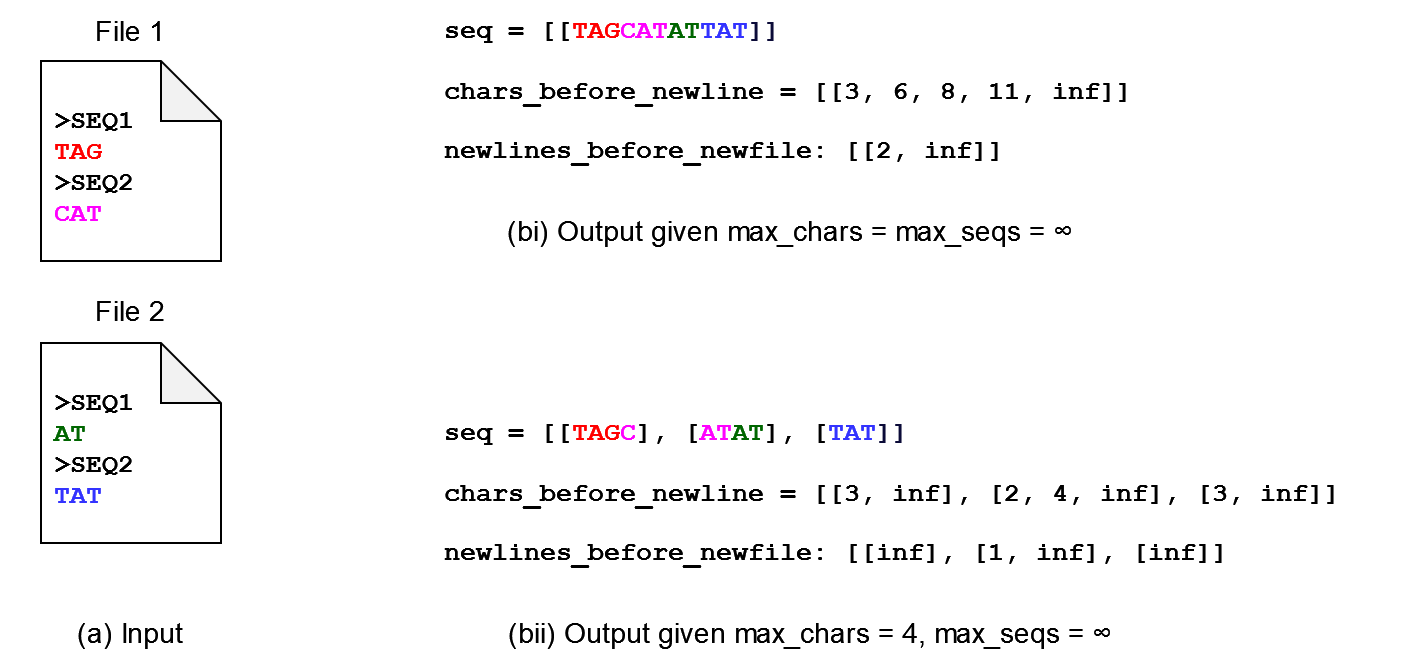
\includegraphics[width=\textwidth]{images/FastaqParser.png}
  \caption{(a) The input FASTA/FASTQ files with the sequences. (b) Outputs of the custom parser. In (bi) the entirety of the input in a single batch is read, whereas three batches are needed in (bii) since the maximum characters per batch is four. Sequences are color coded for easier interpretation.}\label{fig:FastaqParser}
\end{figure}

As a result of more logic involved with this parser, the performance is usually a bit slower than kseq++.
To test this, a FASTA file containing the human genome\footnote{\url{https://www.ncbi.nlm.nih.gov/projects/genome/guide/human/index.shtml}}\footnote{\url{https://ftp.ncbi.nlm.nih.gov/refseq/H_sapiens/annotation/GRCh38_latest/refseq_identifiers/GRCh38_latest_genomic.fna.gz}} and a FASTQ file from a study of early-life microbiota construction\footnote{\url{https://www.ebi.ac.uk/ena/browser/view/PRJEB32631}}\footnote{\url{ftp://ftp.sra.ebi.ac.uk/vol1/fastq/ERR340/004/ERR3404624/ERR3404624_1.fastq.gz}}~\cite{ecoli_genomes_3} were used.
The results and sizes of the files are shown in Table~\ref{tab:KlibVsReklib} and show that kseq++ is usually faster, especially for unzipped FASTA files.
These results were run on the Mahti supercomputer, whose specifications are discussed in Chapter~\ref{ch:Results}.
For decompression, zlib\footnote{\url{https://github.com/madler/zlib}} is used, the same as kseq++.
However, when parsing FASTQ, kseqpp\_REad is very comparable and since most of what the algorithm will be parsing are FASTQ files, as this use case deals with reads and not genomes, the performance drop is acceptable.
One disadvantage of kseqpp\_REad is that the title and quality string information are lost, so it cannot be applied to all workflows.

\begin{table}[]
\centering
\caption{Benchmarking results of kseq++ vs kseq++\_REad when parsing FASTA and FASTQ files in both zipped and unzipped formats. These values are averaged over 5 runs.}\label{tab:KlibVsReklib}
\resizebox{\textwidth}{!}{%
  \begin{tabular}{@{}lllll@{}}
  \toprule
                          & FASTA (2.2 GB)        & FASTA-zipped (928 MB) & FASTQ (3.1 GB)   & FASTQ-zipped (928 MB) \\ \midrule
  kseq++ time             & 2.2s                  & 13.5s                 & 3.7s             & 15.3s    \\
  kseq++ throughput       & 1024 MB/s             & 68 MB/s               & 838 MB/s         & 61 MB/s    \\
  kseq++\_REad time       & 4.2s                  & 15.2s                 & 4.1s             & 15.7s    \\
  kseq++\_REad throughput & 523 MB/s              & 61 MB/s               & 756 MB/s         & 59 MB/s    \\ \bottomrule
  \end{tabular}
}
\end{table}

\subsection{Preprocessing}

There are 2 steps for preprocessing the dataset.
The first is to bitpack it.
This means that the algorithm scans through the sequence produced by the previous step and converts $A$s to 0s, $C$s to 1s, $G$s to 2s and $T$s to 3s.
In binary, these can be represented with just 2-bit per character.
Thus, a u64 vector is created and the characters are packed in this vector in their original order.
This pass can be done in parallel, such that each thread processes the same amount of characters rounded to the nearest index which is a multiple of 64.
For example, given 200 characters, and 2 threads, thread 0 would process characters from 0 to 128, while thread 1 would process the rest.
In this small example, the ratio between the work done by the two threads is significant, as one thread does almost twice as much: $128 / (200 - 72) = 1.78$.
However, given that the number of characters in this case is in the order of millions or billions, one can say that each thread does the same amount of work.

During the same pass as bit-packing, another boolean vector of invalid characters is filled.
An invalid character is one which is not in the alphabet $ACGT$.
At the start, this vector is filled with 0s.
When an invalid character is seen in the sequence at an index $i$, the value of the invalid characters vector at index $i$ is set to 1.
Since this work is done in the same pass as bit-packing, it is also done in parallel, with the bitvector reserved beforehand.
Rather than a vector of booleans, in the implementation a vector of characters is used, as it was found to be faster.
When an invalid character is found, it is represented as if it were an A when it is bit packed, that is, as $00$.

The last preprocessing step is building the positions vector.
As discussed before, if a sequence has $C$ characters, then it has $C - k + 1$ $k$-mers.
The positions are thus u64s which represent the indexes in this sequence where a $k$-mer starts, and the next k characters, that index included, will be considered as a $k$-mer.
To do this position building, the chars\_before\_newline created in the parsing phase are used.
The positions can be generated with a single pass over this vector.
Figure~\ref{fig:Preprocessing1} shows an example of the preprocessing outputs discussed in this subsection.

\begin{figure}[t]
  \centering
  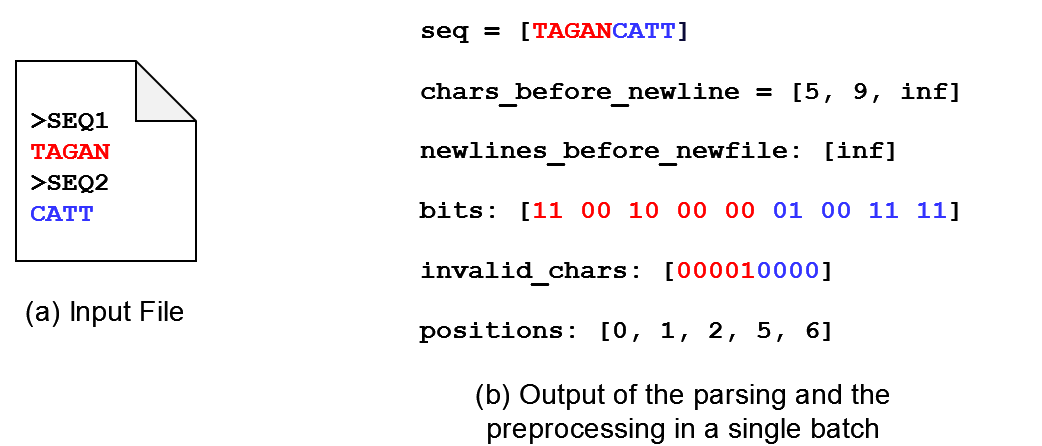
\includegraphics[width=0.8\textwidth]{images/Preprocessing1.png}
  \caption{An example of parsing and preprocessing in a single batch with the maximum characters per batch being $\infty$} \label{fig:Preprocessing1}
\end{figure}

The algorithm uses batching, so that each batch can only have a maximum number of characters and a maximum number of new sequences, whichever is reached first.
Since batching is being used, trouble would ensue if batching breaks a sequence in half, since characters may be shared between $k$-mers.
Hence the final $k-1$ characters must be copied from the previous batch to the start of the new batch in order not to miss any $k$-mers.
The amount may be less than this, as there is only a need for copying if the batching breaks the $k$-mers.
Figure~\ref{fig:Preprocessing2} shows an example where one needs to copy, and a case where copying is unnecessary.
There are also middle cases where one may need to copy some characters but less than $k-1$ characters.
This happens when the batching cuts off a sequence at its beginning, that is, before k characters have been parsed from it.
Copying is done in the parsing step, the first step discussed, so the rest of the components are oblivious to this step.

\begin{figure}[t]
  \centering
  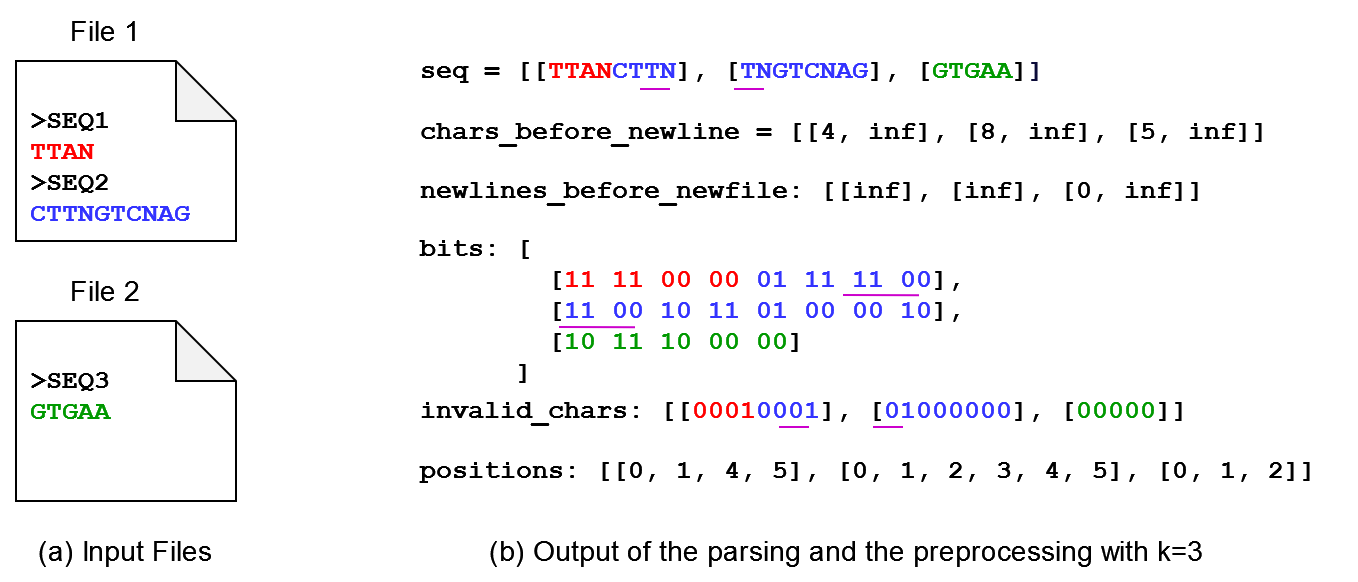
\includegraphics[width=\textwidth]{images/Preprocessing2.png}
  \caption{A second example of preprocessing, with the maximum characters per batch being 8. Notice how the string gets broken between the first and second batch, but not between the second and third. Overlapping areas have been marked with purple lines.}\label{fig:Preprocessing2}
\end{figure}

\subsection{Searching}

The index searching algorithm was discussed in Section~\ref{sec:SBWTQuerying}.
The only difference now is that the processing is done on the GPU.
Remember that the SBWT, the Poppys and the key-$k$-mer marks are already copied to the GPU.
Now the bit-packed sequence and the positions also need to be copied there.
Thus, each thread on the GPU handles a single position, since there is no relation between one $k$-mer search and the next.
As an optimisation, to save memory, and perform less memory accesses, one can overwrite the u64s of the positions with the u64s of the search result.
After this, the results can be copied back to memory and written to disk.
This GPU search function was created previously~\cite{Harri} but is now refactored and used in the new solution.
One change that this thesis has made to the previous implementation is to make it possible to query for $k > 32$ by always querying global GPU memory for the next two bits, rather than first storing the entire $k$-mer into a u64 and then querying that.
Although the performance difference between the previous and new kernel was not measured in isolation, this change was not shown to impact the overall performance of the algorithm from start to finish, since the kernel is only a small part of the bigger picture.

One more optimisation to searching which was used in previous works is presearching \cite{Presearch, SBWT, Harri}.
This is done right after loading the SBWT to the GPU, however, it was chosen to discuss it now in order not to confuse the reader with too much disjoint information at the beginning.
The notion behind presearching is that one can search for the first part of the $k$-mers beforehand, store these in memory, so then rather than recomputing these, they can be loaded from memory and continue the search continues from there.
To do this presearching, the left and right pointers are moved forward by a certain amount $k_p$ for every permutation of a $k_p$-mer.
Thus, given for example $k_p=2$, the combinations are: $AA, AC, AG, AT, CA, CC, \ldots, TG, TT$.
Represented as binary, they become: $0000, 0001, 0010, 0011, 0100, 0101, \ldots, 1110, 1111$.
The decimal representation is then: $0, 1, 2, 3, 4, \ldots, 14, 15$.
Thus note that these can be used as the indexes to both store and later retrieve the presearched left and right pointers for $k_p$.

In the example, 16 memory spaces are needed.
More generally, $4^{k_p}$ are needed for each of the left and right pointers, where each memory space contains a u64.
Thus, the final formula for the total number of bits to store the presearch results is \[4^{k_p} \times 64 \times 2 \quad \mathit{bits}.\]
Ideally, one would presearch with $k_p = k$, however, the memory requirements for this would be massive, as the formula is exponential on $k_p$.
If $k_p=k=31$, this would require $4^{31} * 64 * 2 / 8 / 1024 ^ 3 \approx 9$ billion GB.
As a result, similar to the previous GPU method~\cite{Harri}, $k_p=12$ is used.
With this, 250MB of data are needed in total for the presearch data.
Algorithm~\ref{alg:SearchWithPresearch} shows the final search algorithm.

\begin{algorithm}
	\KwIn{\newline
    A sequence $S = c_1, c_2, \ldots, c_k$ \newline
    Bitvectors $b_A, b_C, b_G, b_T$
    c-map $C$
    Presearch size $k_p$
    Presearch maps $presearch_{\mathit{left}}$ and $presearch_{right}$
	}
  $\mathit{left}$ = $presearch_{\mathit{left}}[c_1, \ldots, c_{k_p}]$

  $\mathit{right}$ = $\mathit{presearch}_{right}[c_1, \ldots, c_{k_p}]$

  \ForEach{c \textbf{in} S[($c_{k_p} + 1$) \ldots k]}{
    $\mathit{left}$ = $C[c]$ + rank ($b_c$, $left$)

    $\mathit{right}$ = $C[c]$ + rank ($b_c$, $right + 1$) \-- 1

    \If{$\mathit{left}$ > $\mathit{right}$} {\
      \textbf{return} not found
    }
  }

  \textbf{return} $left$

  \caption{Index Search function with presearch.}\label{alg:SearchWithPresearch}
\end{algorithm}

\subsection{Results Printing}

For results printing, there are three output formats, but programmatically they follow the same interface.
This means that in general, they all print to a memory buffer first and then these buffers are printed to disk.
Printing to buffers is done in parallel, meaning that each thread has an equal amount of indexes to print and each thread prints to its own equally sized buffer, and then the buffers are printed to disk sequentially.
The reason it was opted to parallelise this pass, rather than simply printing to disk, is because of the conversions which need to be done, from the binary representation in memory, to the representation on disk.
For this step, the search results are used, the chars\_before\_newline to know where to split each sequence, the seqs\_before\_newfile to know when the algorithm needs to open the next file, and the invalid characters list to differentiate these from the characters which were not found.
The feature to differentiate invalid characters from the not-founds is not found in Themisto or its precursors, and is hence another new contribution.

Next, each output format is discussed.
Figure~\ref{fig:IndexResultsPrinting} serves as a good visualisation of how the characters are written to disk.
It is important to note that the only implementation difference between these formats is how they print each value.
The available values which they can print are the following: a found index, a not-found index, an invalid character, or a newline.
The first to consider is the ASCII format, where the indexes are printed as a space-separated list of values.
The values for the indexes are simply u64s, so they can be printed as their ASCII counterparts.
The not-found values are represented as $-1$, invalid characters as $-2$, and newline values as the expected line feed character \textit{\textbackslash n}.
This format was the one that saw the largest benefit from parallelisation, as the operation to convert from binary to ASCII, especially for larger numbers, takes significant CPU time, due to the need of performing many division and modulus operations which are computationally expensive.
In order to convert from binary to ASCII, the algorithm created by James Anhalt\footnote{\url{https://github.com/jeaiii/itoa}} is used.
This was benchmarked on a dummy dataset internally against the \textit{to\_string} algorithm from the GCC C++ standard library and against the \textit{format\_decimal} algorithm by \textit{fmt}\footnote{\url{https://github.com/fmtlib/fmt}} library and it was found that the algorithm by Anhalt was significantly faster than these alternatives.
It is also the fastest algorithm in other benchmarks\footnote{\url{https://jeaiii.github.io/itoa/}}.
No detail will be given as to how the u64 to ASCII algorithm works and what differentiates it from other algorithms, as this problem is a deep rabbit hole and could make for its own thesis.

\begin{figure}[t]
  \centering
  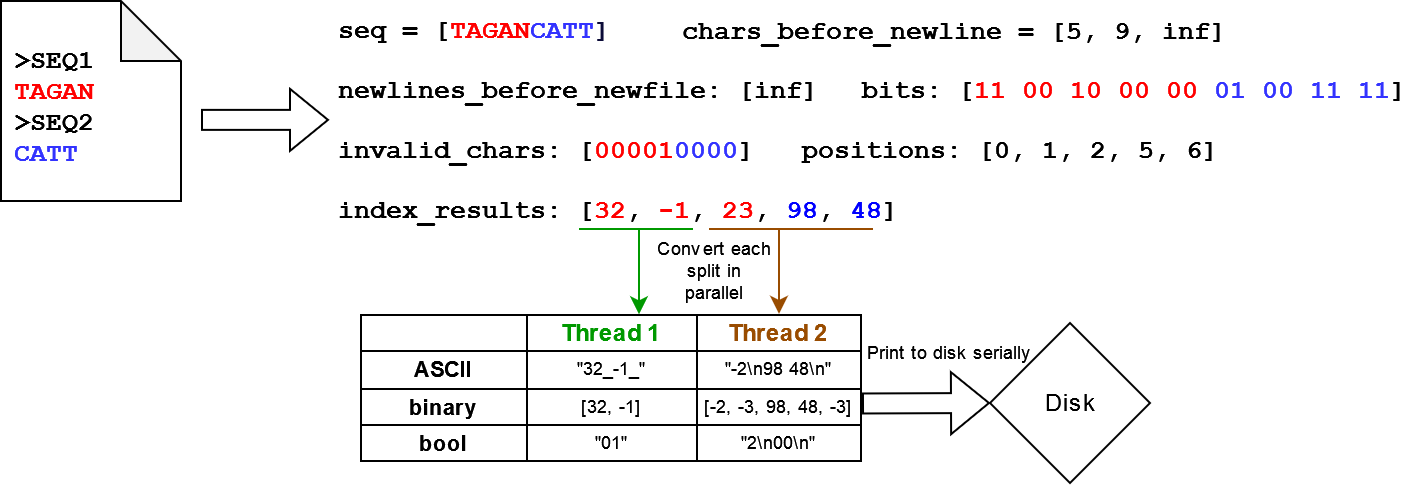
\includegraphics[width=\textwidth]{images/IndexResultsPrinting.png}
  \caption{The results printing pipeline from FASTA/FASTQ files to printing to disk in a single batch. The parallelisation of this is also visualised. For the ASCII and bool formats, these use usual 8-bit ASCII characters for their representation, whereas for the binary format uses a contiguous array of u64s.}\label{fig:IndexResultsPrinting}
\end{figure}

The second format is the binary format.
In this format, each element that is printed takes 8 bytes, as everything is printed as a u64.
Results are printed as they are.
Meanwhile, not-found values are printed as the maximum u64 value, that is, $2^{64}$, invalid values are printed as $2^{64} - 1$, and newlines are printed as the $2^{64} - 2$.
In C++, unsigned integers loop back when they overflow, so that one can say that the values for not-founds, invalids and newlines are $-1$, $-2$, and $-3$ respectively.
This method would be faster and with less memory requirements than the ASCII format if most of the indexes contain more than 8 bytes.
The ASCII format requires at most 20 bits for each character, since the maximum value of u64 is 20 characters long, plus another character for the whitespace character which separates the values.
However, as will be seen in Chapter~\ref{ch:Results}, while not drastically slower than the ASCII format, this method ends up taking a lot more space, since the indexes are usually not too large.

The last format is dubbed the boolean format.
In this format, the sequences are separated with newlines, as in the ASCII format.
However, for the values, a single byte is used.
For the found values, the ASCII character for 0 is printed, then the not-founds are represented with a 1 and the invalids are represented with a 2.
This makes it the smallest format and also also the fastest to print, at the cost of losing the index information, that is, where the $k$-mer is found within the SBWT.
As a result, it is not suitable for the second phase, since the indexes are needed.
However, it is the best format for users who simply want to know if the $k$-mers of their sample exist within the SBWT or not.
